
% Inbuilt themes in beamer
\documentclass[aspectratio=169]{beamer}
\usepackage{graphicx}
% Theme choice:
\usetheme{CambridgeUS}

% Title page details: 
\title{Econometrics Discussion Section 2: Experiments} 
\author{John Green}
\date{Spring 2024}


\begin{document}

% Title page
\begin{frame}
    \titlepage 
\end{frame}

% Outline frame
\begin{frame}{Experiments}
    \begin{itemize}
        \item Why do economists like \textit{experiments}?
        \begin{itemize}
            \item Experiments provide \textit{exogeneous variation} via the treatment variable: they solve the endogeneity problem and let us estimate a causal effect (eg the ``treatment effect'')
            \item A ``randomized control trial'' (RCT) is the gold standard: assign treatment $D$ randomly, and compare $E[Y|D=1,X] - E[Y|D=0,X]$ to get the treatment effect of $D$ on $Y$
        \end{itemize}
        \item \textit{Potential outcomes} framework identifies for each individual:
        \begin{itemize}
            \item $Y_1$: the outcome if treated
            \item $Y_0$: the outcome if untreated
            \item The \textit{treatment effect} is $Y_1 - Y_0$
        \end{itemize}
        \item But of course, for each individual we only observe one outcome! So we need to be clever to estimate this...
    \end{itemize}
\end{frame}

\begin{frame}{Average treatment effect}
    \begin{itemize}
        \item Through OLS we can recover the average treatment effect, or ATE
        \item If we have an RCT then our model is simply:
        \begin{equation}
            Y = \beta_0 + \beta_1 D_i + \beta_2 X_i \epsilon_i
        \end{equation}
        where $X_i$ are control variables and $\hat{\beta_1} = E[Y|D=1] - E[Y|D=0]$ is the ATE (differences estimator)
        \item Controlling for $X_i$ is always helpful, but is crucial if the assignment was randomized based on some controls (why?)
        \item If we expect the effect to also depend on $X_i$, we need to include interactions
    \end{itemize}
\end{frame}

\begin{frame}{Potential problems}
    \begin{itemize}
        \item Issues with the experiment:
        \begin{itemize}
            \item Imperfect randomization (causes correlation with error term)
            \item Partial compliance (use an IV)
            \item Attrition (sample selection bias)
            \item Experimental effects
        \end{itemize}
        \item External validity threats:
        \begin{itemize}
            \item Non-representative sample
            \item Non-representative treatment  
            \item GE effects
        \end{itemize}
    \end{itemize}
\end{frame}

\begin{frame}{Quasi-experiments}
    \begin{itemize}
        \item Economic experiments are rare:
        \begin{itemize}
            \item Expensive
            \item Time-consuming
            \item Might be unethical
        \end{itemize}
        \item So, we often look for a \textit{natural experiment} or \textit{quasi-experiment}
        \item In a natural experiment the treatment is assigned semi-randomly by some mechanism besides an explicit RCT design
        \begin{itemize}
            \item Treatment is semi-random (minimum wage changes in NJ, not in NY)
            \item Some other factor $Z$ influences receipt of treatment $D$, so is an instrument
            \item Example: section 8 housing vouchers
        \end{itemize}
    \end{itemize}
\end{frame}

\begin{frame}{Natural experiment estiamtors}
    \begin{itemize}
        \item Diff-in-diff: compare two groups in (at least) two time periods where one group gets a treatment
        \item IV Estimation
        \item Regression discontinuity (sharp)
        \item Fuzzy discontinuity
    \end{itemize}
\end{frame}

\begin{frame}{Big data and machine learning}
    \begin{itemize}
        \item ``Big data'' are just data sets with many (millions) of observations $n$ or many (thousands) of variables $k$
        \begin{itemize}
            \item Might even be the case that $k > n$ and OLS is not possible
        \end{itemize}
        \item Forget about causation and just think about prediction
        \begin{itemize}
            \item Train a model on \textit{training data} and test it on \textit{test data}
        \end{itemize}
    \end{itemize}
\end{frame}

\begin{frame}{Prediction}
    \begin{itemize}
        \item Standardize all our data to be mean 0 and variance 1 so that the intercept drops out, and our model is:
        $$
        Y_i=\beta_1 X_{1 i}+\beta_2 X_{2 i}+\ldots+\beta_k X_{k i}+U_i
        $$
        \item The ``oracle prediction'' is the best possible predictor, ie that which minimizes the mean squared percentage error on the out-of-sample data:
        $$
        \text{MSPE} = \mathbb{E}\left[Y^{OOS}-\hat{Y}\left(X^{OOS}\right)\right]^2
        $$
    \end{itemize}
\end{frame}

\begin{frame}{Oracle error}
    \begin{itemize}
        \item Our standard OLS model \textit{does not} give us the oracle prediction because we have to estimate our coefficients, which introduce additional uncertainty
        $$
        \text{MSPE}_{O L S} \cong\left(1+\frac{k}{n}\right) \sigma_u^2
        $$
        \begin{itemize}
            \item So $\text{MSPE}_{O L S}$ is decreasing in sample size but increasing in predictors
        \end{itemize}
        \item We get around this by allowing for bias in our coefficient estimates
        \item Do so with a shrinkage estimator (like James-Stein) which accepts some bias in exchange for higher variance, which gives us a better OOS prediction:
        $$
        \hat{\beta}^{J S}=c \hat{\beta}
        $$

    \end{itemize}
\end{frame}

\begin{frame}{Bias-variance tradeoff}
    \begin{itemize}
        \item In general, we face a tradeoff between bias and variance
        \begin{itemize}
            \item Remember that OLS is unbiased!
        \end{itemize} 
        \item Flexible model has low bias, but it will be more sensitive to noise and have a higher variance
        \item If number of regressors is large, then an increase in bias which reduces variance may reduce the MSPE and thus be ``worth it'' 
    \end{itemize}
\end{frame}


% \begin{frame}
%     \centering
%     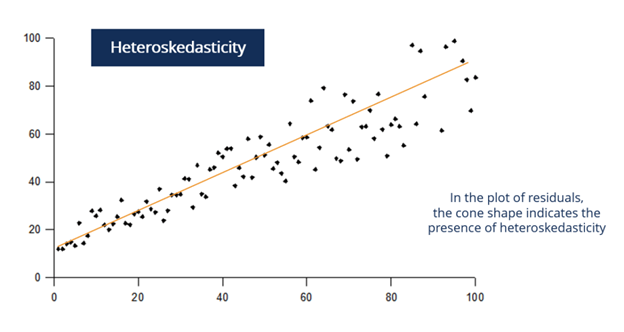
\includegraphics[width = .75\textwidth,keepaspectratio]{./figs/heteroskedasticity.png}
% \end{frame}


\end{document}